\documentclass[11pt,oneside,a4paper,article]{memoir}
\usepackage{fontspec}
\usepackage{graphicx}
\usepackage[unicode=true,xetex,colorlinks=true,linkcolor=blue,urlcolor=blue,bookmarksnumbered=true,bookmarksdepth=3]{hyperref}

%%%%%%%%%%%%%%%%%%%%%%%%%%%%%%%%%%%%%%%%%%%%%%%%%%%%%%%
%%%%%%%%%%%%%%%%%%% How to typeset %%%%%%%%%%%%%%%%%%%%
%%%%%%%%%%%%%%%%%%%%%%%%%%%%%%%%%%%%%%%%%%%%%%%%%%%%%%%

%% This file must be run through xelatex

%% The "Linux Libertine O" font must be accessible to xelatex.
%%
%% On Ubuntu Linux, this font can be installed thus:
%%
%% sudo apt install fonts-linuxlibertine


%%%%%%%%%%%%%%%%%%%%%%%%%%%%%%%%%%%%%%%%%%%%%%%%%%%%%%%
%%%%%%%%%%%%%%%%%%%% Configuration %%%%%%%%%%%%%%%%%%%%
%%%%%%%%%%%%%%%%%%%%%%%%%%%%%%%%%%%%%%%%%%%%%%%%%%%%%%%

%%% Fonts %%%
\setmainfont[Ligatures=TeX]{Linux Libertine O}

\newfontfamily{\mainnolig}{Linux Libertine O}
\newcommand{\q}{{\mainnolig '}}

%%% Page layout %%%
\settypeblocksize{247mm}{160mm}{*}
\setlrmargins{*}{*}{1}
\setulmargins{*}{*}{1}
\checkandfixthelayout

%%% Hyperref (Information in PDF) %%%
\hypersetup{
unicode=true,
pdfauthor={Claus Tøndering},
pdftitle={Resources Website -- Adminstrator's Guide}
}

%%% Lists %%%
\tightlists

%%% Allow extra space between words %%%
\sloppy


%%% Font matter %%%
\title{Resources Website -- Administrator's Guide}
\author{Claus Tøndering}
\date{19 September 2023}


\begin{document}
\maketitle


%%%%%%%%%%%%%%%%%%%%%%%%%%%%%%%%%%%%%%%%%%%%%%%%%%%%%%
%%%%%%%%%%%%%%%%%%%% Introduction %%%%%%%%%%%%%%%%%%%%
\chapter{Introduction}

The ``Resources Website'' or ``Picture Database'' is a collection of photographs relating to areas
in ancient Israel and the surrounding countries.

Anybody can view and download the pictures at \url{https://resources.learner.bible}. Users with an
account on the web site can log in and manage the collection of pictures. The description in the
following sections assumes that you are logged in.

Most of the web pages have associated help information. Click the ``? Help'' button to get
information about the current page. This document does not include information that can be found in
the help system.

\section{Copyright and License}

The pictures are are available under a \emph{Creative Commons Attribution-NonCommercial-ShareAlike 3.0
  Unported License.} Details can be found by clicking ``Copyright and license'' in the left panel of
the website.

%%%%%%%%%%%%%%%%%%%%%%%%%%%%%%%%%%%%%%%%%%%%%%%%%%%%%%%%
%%%%%%%%%%%%%%%%%%%% Classification %%%%%%%%%%%%%%%%%%%%
\chapter{Classification}

The pictures are classified in four classes:

\begin{itemize}
\item \emph{Place:} The location where the picture was taken; for example, ``Jerusalem'' or
  ``Ephesus''.
\item \emph{Culture:} The theme of the picture; for example, ``Landscapes'' or ``Cosmetics''. A
  picture can have more than one theme.
\item \emph{Period:} Time period of the items in the picture; for example, ``Early bronze (3300-2000
  BC)'' or ``Modern''. A picture can belong to more than one period.
\item \emph{Resolution type:} The resolution of the picture and size of the file; for example,
  ``Medium (500KB - 6MB)''.
\end{itemize}

Furthermore, each picture has a descriptive text in Danish and/or English.


%%%%%%%%%%%%%%%%%%%%%%%%%%%%%%%%%%%%%%%%%%%%%%%%%%%%%%%%%
%%%%%%%%%%%%%%%%%%%% Adding Pictures %%%%%%%%%%%%%%%%%%%%
\chapter{Adding Pictures}

Adding a picture to the system is a two-step process. First the picture must be \emph{uploaded},
then it must be \emph{published}.

\Needspace*{4cm}%
The name of the picture file is important, because it relates directly to the classification of the
picture. The file name must have this structure:

\begin{center}
<place or culture>\_<periods>\_<picture number>\_<resolution>.jpg
\end{center}

\noindent
where

\begin{itemize}
\item <place or culture> is a point-separated list of numbers identifying the place and culture
  classifications\footnote{Although place and culture are separate categories, they share a number
    space.} of the picture,
\item <periods> is a point-separated list of one numbers identifying the period classifications of the
  picture,
\item <picture number> is a unique number in a range assigned to the photographer,
\item <resolution> is the character H, M or L, identifying High (>~6MB), Medium (500KB-6MB) or Low
  (<~500KB).
\end{itemize}

The numbers for place, culture and period can be found under the menu ``Edit category
descriptions''. The number range for each photographer can be found under the menu ``Edit photographers''.

For example, a file name such as ``272.2301\_8.15\_627\_M.jpg'' would be related to place and culture
numbers 272 and 2301, periods numbers 8 and 15, have picture number 627, and have Medium resolution.

The system accepts .jpg and .png files.

Uploading is done through the ``Upload pictures'' menu. When a picture has been uploaded, it enters
the ``Unpublished'' state. Unpublished pictures can be seen through the ``Manage unpublished
pictures'' menu.

%%%%%%%%%%%%%%%%%%%%%%%%%%%%%%%%%%%%%%%%%%%%%%%%%%%%%%%%%%%%%%%%%%%%%%%%%%%%
%%%%%%%%%%%%%%%%%%%% Connection to Bible Online Learner %%%%%%%%%%%%%%%%%%%%
\chapter{Connection to Bible Online Learner}

There are two sets of connections from the resources website to Bible Online Learner (Bible OL).

Firstly, references to Old Testament passages in the descriptive text of a picture are made available to Bible
OL. If a user looks up a bible passage in Bible OL and checks the ``Show link icons'' checkbox,
links to the relevant picture in the resources website will be shown as a P in a circle:

\begin{center}
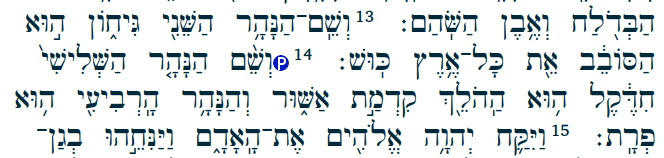
\includegraphics[width=10cm]{picture_link.png}
\end{center}

Secondly, the resources website can provide URLs connected to specific Old Testament passages.
Through the ``Edit Bible reference URLs'' menu in the resources website, a URL and an icon can be
associated with a Bible reference. The chosen icon will appear in the same way as the P in the above
illustration.

The available icons here are the letters D, V and U, which are intended to identify documents,
videos and other URLs, respectively.

Note that at present only Old Testament references are handled.

Bible OL normally retrieves information from the resources website once an hour, so there will be a
time lapse of up to one hour between the time when a Bible reference is configured in the resources
website and the information is available in the Bible OL website. Bible OL retrieves the information
by accessing the URLs \texttt{https://resources.learner.bible/jsonrefs.php} and
\texttt{https://resources.learner.bible/jsonrefs.php}, respectively.

\end{document}

% Local Variables:
% mode: latex
% ispell-dictionary: "british-ize"
% ispell-extra-args: ("--home-dir=/home/claus/Projects/BibleOL/techdoc")
% eval: (auto-fill-mode 1)
% End:
